\documentclass[11pt]{article}

\usepackage[utf8]{inputenc}
\usepackage[T1]{fontenc}
\usepackage{lmodern}
\usepackage{amsmath,amssymb}
\usepackage{booktabs}
\usepackage{tabularx}
\usepackage{array}
\usepackage{enumitem}
\usepackage{geometry}
\usepackage{tikz}
\usepackage[numbers]{natbib}
\usepackage{hyperref}
\hypersetup{hidelinks}

\geometry{margin=1in}
\setlength{\parindent}{0pt}
\setlength{\parskip}{0.7em}
\newcolumntype{Y}{>{\raggedright\arraybackslash}X}

\title{From Free-Energy Loops in the Brain to Human Values}
\author{Gunnar Zarncke, aintelope}
\date{May 20, 2026}

\begin{document}
\maketitle

\begin{abstract}
\citet{zarncke2025stratification} catalogues fifteen free-energy-minimising loops in the vertebrate brain, ordered by evolutionary age in a companion ledger.
Each loop closes a prediction-error feedback and projects into one or more neuromodulatory or salience ``hubs'' that broadcast precision weights.
Here we introduce a loop-hub-control-value (LHCV) model:
an architectural proposal in which a small set of hubs transforms high-dimensional error vectors into low-bandwidth scalars,
which function as control relevance proxies and are read out, through development and context, as human value tags.
We (i) formalise three transfer steps, loop $\to$ hub, hub $\to$ control relevance proxy, and control relevance proxy $\dashrightarrow$ value readout;
(ii) compile an empirical mapping between hubs, control relevance proxies, and typical value readouts, drawing on the stratified ledger;
and (iii) outline falsifiable predictions.
\end{abstract}

\section{Architecture}

Biological agents cannot transmit every prediction error upstream; long-range bandwidth is constrained by wiring and metabolic costs. Evolution addresses this with hub bottlenecks: mid-brain nuclei and limbic structures that compress high-dimensional loop errors into slow neuromodulatory scalars.
The upstream loop inventory follows the stratified free-energy ledger of \citet{zarncke2025stratification}; LHCV specifies how those loop errors are bottlenecked, control-relevant, and eventually read out as values.

In the loop--hub--control--value (LHCV) model, those scalars serve two roles at different timescales. \emph{Immediately}, they act as control relevance proxies that steer policy---modulating attention, precision, learning rate, exploration, inhibition, and action priors. \emph{Developmentally}, overlapping proxy histories are decoded---via language, social feedback, memory, and self-model---into stabilized human value readouts.

The architecture is a four-stage pipeline:
\[
\mathrm{L} \to \mathrm{H} \to \mathrm{C} \dashrightarrow \mathrm{V},
\]
where L denotes free-energy loops, H denotes hub bottlenecks, C denotes control relevance proxies, and V denotes learned value readouts. The dashed arrow marks contextual mediation, not a direct anatomical projection.

\begin{figure}[ht]
\centering
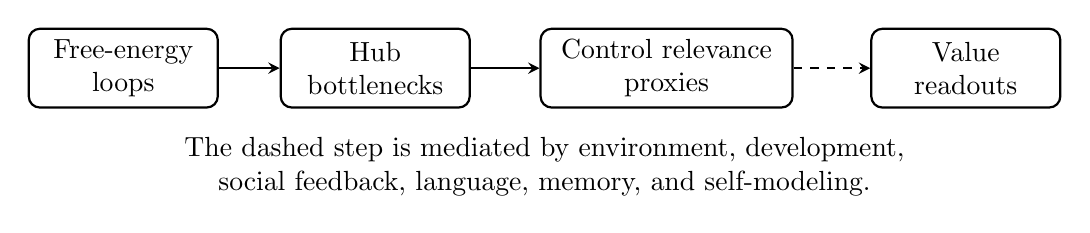
\begin{tikzpicture}[>=stealth,thick]
  \node[draw,rounded corners,align=center,minimum width=2.4cm,minimum height=1.0cm] (loops) at (0,0) {Free-energy\\loops};
  \node[draw,rounded corners,align=center,minimum width=2.4cm,minimum height=1.0cm] (hubs) at (3.2,0) {Hub\\bottlenecks};
  \node[draw,rounded corners,align=center,minimum width=3.2cm,minimum height=1.0cm] (control) at (6.9,0) {Control relevance\\proxies};
  \node[draw,rounded corners,align=center,minimum width=2.4cm,minimum height=1.0cm] (values) at (10.7,0) {Value\\readouts};
  \draw[->] (loops) -- (hubs);
  \draw[->] (hubs) -- (control);
  \draw[->,dashed] (control) -- (values);
  \node[align=center,text width=9.5cm] at (5.35,-1.25) {The dashed step is mediated by environment, development, social feedback, language, memory, and self-modeling.};
\end{tikzpicture}
\caption{The LHCV pipeline: free-energy loops compress through hub bottlenecks into control relevance proxies, which are read out as human values under developmental and environmental mediation.}
\end{figure}

\section{Formal Skeleton of the LHCV Model}

We now instantiate each step.

\textbf{Error compression.} Each loop $i$ in the stratified ledger \cite{zarncke2025stratification} produces an error vector $\epsilon_i(t) \in \mathbb{R}^{d_i}$. A hub $h$ receives a weighted sum over incoming loops
\begin{equation}
  s_h(t) = \sigma\left(\sum_{i\in I(h)} w_{ih} \lVert \epsilon_i(t) \rVert_p\right),
\end{equation}
where $\sigma$ is a saturating non-linearity and $w_{ih}$ are learned transfer weights.

\textbf{Control relevance proxies.} Hub scalars map to control relevance proxies,
\begin{equation}
  c_h(t) = g_h\big(s_h(t), z_t, a_t\big),
\end{equation}
where $z_t$ is the current learned state and $a_t$ denotes the current action context. A control relevance proxy is a compressed signal about where control is needed, valuable, or failing: threat, damage, uncertainty, metabolic deficit, social exclusion, caregiver need, opportunity, or policy regret. These proxies can modulate attention, precision, memory writing, exploration, inhibition, learning rate, and action priors.

One simple policy-level readout is
\begin{equation}
  \pi(a_t \mid z_t, c_t)
  \propto
  \exp\left(Q_\theta(z_t,a_t) + \sum_h \lambda_h c_h(t)\,\phi_h(z_t,a_t)\right),
\end{equation}
where $\phi_h$ selects the action features affected by proxy $h$ and $\lambda_h$ controls the strength of the corresponding policy bias.

\textbf{Value readout.} A cortical and social decoder $D$ maps hub-shaped control histories into symbolic values $V = \{v_1, \ldots, v_m\}$ via
\begin{equation}
  P\left(v_k \mid \{c_h\}_h, e_t\right)
  = \operatorname{softmax}_k\left(\beta_k + \sum_h \alpha_{kh}(e_t)c_h\right),
\end{equation}
where $e_t$ summarizes the environment-mediated developmental context: learned concepts, social feedback, language, memory, and self-modeling. The coefficients $\alpha_{kh}$ are contextually gated by attention and task set. This is the formal location of the dashed $\mathrm{C}\dashrightarrow\mathrm{V}$ step.

\textbf{Interpretive note.} The LHCV model therefore does not claim that ``PAG represents protection'' or ``ACC represents justice.'' It claims that nocifensive, conflict, salience, and precision signals make protection-like, justice-like, care-like, and truth-like abstractions easier to learn and stabilize in ordinary developmental environments.

\section{Empirical Hub-Control-Value Map}

Table~\ref{tab:lhcv-map} lists the hubs, the principal loops that feed them, the primary control relevance proxies, and typical downstream value readouts. The table should be read as a hypothesis generator. The value column is downstream and mediated; the control relevance proxy column is the more direct biological claim.

\begin{table}[ht]
\centering
\scriptsize
\begin{tabularx}{\textwidth}{p{0.19\textwidth} p{0.20\textwidth} Y Y}
\toprule
\textbf{Hub} & \textbf{Dominant upstream loops} & \textbf{Primary control relevance proxy} & \textbf{Typical value readouts} \\
\midrule
Periaqueductal Gray (PAG) & Threat-pain; Pavlovian threat loop & Nocifensive urgency, defensive inhibition, protection pressure & Protection, non-suffering, bodily safety \\
Ventral Tegmental Area (VTA) & Curiosity; valuation regret & Exploration, novelty, reward-prediction update & Learning, curiosity, discovery, diversity \\
Locus Coeruleus (LC) & Precision-timing & Arousal, uncertainty, precision, task urgency & Achievement, vigilance, responsibility \\
Nucleus Accumbens (NAcc) & Valuation-agency & Approach, appetitive salience, agency-contingent reward & Happiness, motivation, agency \\
Orbitofrontal Cortex (OFC) & Policy-regret valuation & Counterfactual value, regret, expected outcome & Appraisal, prudence, hedonics \\
Hypothalamus & Metabolic; steroidal timing & Metabolic, thermoregulatory, and caregiving regulation & Longevity, care, nurturance \\
HPG axis & Steroidal timing & Reproductive timing, mating effort, status-sensitive endocrine allocation & Reputation, mating, life-history strategy \\
Insula & Metabolic; morphological repair & Interoceptive error, disgust, boundary salience & Purity, fairness, self-protection \\
Anterior Cingulate Cortex (ACC) & Coalition entropy & Conflict, effort, social pain, coalition error & Justice, respect, duty \\
Amygdala & Pavlovian threat tagging & Affective threat, social salience, fear conditioning & Danger, trust, virtue/vice tags \\
Septal Nuclei & Reproductive physiology & Bonding, affiliative reward, social soothing & Loyalty, affiliation \\
Superior Colliculus & Perimeter defence & Orienting, vigilance, defensive spatial prioritization & Situational awareness, nature, truth-like orientation \\
Primary Visual Cortex & Habitat-fit (scene preference)\textsuperscript{\dag} & Scene novelty, aesthetic salience, perceptual compression gain & Beauty \\
\bottomrule
\end{tabularx}
\caption{Hub-control-value correspondences. \textsuperscript{\dag}External twin of metabolic homeostasis in the stratified ledger \cite{zarncke2025stratification}. Value readouts are not claimed to be directly represented in hubs; they are learned downstream from control relevance proxies under environmental and social mediation.}
\label{tab:lhcv-map}
\end{table}

\section{Orphaned Hubs and Candidate Loops}

Although most neuromodulatory hubs receive direct input from an identified free-energy loop in the stratified ledger \cite{zarncke2025stratification}, three sub-hubs in Table~\ref{tab:lhcv-map}--orbitofrontal cortex (OFC), hypothalamo-pituitary-gonadal (HPG) axis, and amygdala--lack a dedicated first-pass hub projection in the present map. We treat them as bottleneck refinements: second-stage processors that reshape upstream error signals onto slower or more specialised control relevance proxies. Below we sketch their provisional computations and outline candidate loops formalised in \citealp{zarncke2025stratification}.

\subsection{Orbitofrontal Cortex (OFC)}

The OFC integrates multi-modal evidence with predicted outcomes to compute a policy-regret signal: the squared discrepancy
\[
  \mathbb{E}\left[(Q^\star - Q)^2\right]
\]
between the best attainable action value $Q^\star$ and the executed value $Q$. This counterfactual loop acts on a timescale of hundreds of milliseconds to seconds, refining valuation updates supplied by ventral striatum and VTA.

\subsection{Hypothalamo-Pituitary-Gonadal (HPG) Axis}

The HPG axis implements neuroendocrine control over fertility and life-history trade-offs. We posit a distinct steroidal timing loop that minimises a deviation term
\[
  \left|S_{\mathrm{steroid}} - \hat{S}\right|,
\]
where $S_{\mathrm{steroid}}$ denotes circulating gonadal hormones and $\hat{S}$ an energy- or age-adjusted set-point. Feedback operates over hours to months, providing a slow but powerful prior on reproductive strategy.

\subsection{Amygdala}

Beyond rapid nocifensive processing in the periaqueductal loop, the basolateral-central amygdala complex assigns socio-emotional salience. We hypothesise a social appraisal loop that reduces entropy over affective threat states,
\[
  H\left(\mathrm{threat}_{\mathrm{aff}}\right),
\]
capturing mid-latency fear conditioning and norm-violation detection.

\section{Predictions}

Because control and value occupy different layers, LHCV yields distinct falsifiers for each:

\begin{enumerate}[leftmargin=*]
  \item Disrupting a hub should first perturb salience, attention, action priors, learning rates, inhibition patterns, and exploration tendencies. Value reports should shift downstream when the relevant learned value concepts depend on those control relevance proxies.
  \item Task contexts that enlarge $\lVert\epsilon_i\rVert$ will modulate control relevance proxies in proportion to $w_{ih}$, and will modulate subjective value ratings only where the corresponding value decoder depends on those proxies.
  \item Agents endowed with an LHCV bottleneck should yield more interpretable policy and preference shifts than agents using flat reward summation when hub or proxy weights are perturbed.
  \item The H$\to$C effect should be more anatomically immediate and cross-context stable than the C$\dashrightarrow$V effect. Developmental history, language, and social environment should explain substantial variance in the value readout from the same control relevance proxy.
\end{enumerate}

\section{Related Research}

\subsection{Loop-Through-Hub Circuitry}

Weiller et al.\ \citep{weiller2022} identify a dual-loop motif in human cortex where dorsal (sequencing) and ventral (conceptual) streams converge on frontal and posterior hubs, forming a closed circuit. Expanding this, Weiller et al.\ \citep{weiller2025} describe a meta-loop in which lateral (external) and medial (internal) dual-loops interact via cross-hub projections, furnishing a substrate for integrating needs and demands.

Lyu et al.\ \citep{lyu2021} provide causal evidence: effective-connectivity analyses reveal a recurrent loop between dorsal and ventral precuneus subdivisions that modulates DMN and fronto-parietal networks as tasks change. These findings validate the LHCV claim that prediction-error messages funnel through hubs before influencing global policy.

\subsection{Hub-Level Precision Weighting}

Predictive-coding theory posits that precision (gain) of error signals is regulated by key hubs. Thalamic work by Kanai and Friston \citep{kanai2015} highlights the pulvinar as a relay that encodes sensory reliability and synchronises relevant cortices, implementing precision control. Human fMRI by Hauser et al.\ \citep{hauser2018} shows unsigned prediction-error signals in dorsal ACC and superior frontal cortex are precision-weighted in a dopamine-dependent manner, underscoring cortical hubs in error salience modulation.

\subsection{Internal Control-External Information Integration}

The salience network, centred on anterior insula and dorsal ACC, mediates switching between internal and external modes \citep{menon2023}. Malfunctions yield aberrant salience attribution, reinforcing its control-allocation role. Complementarily, fronto-striatal loops through ventral striatum and OFC relay dopaminergic reward-prediction signals, aligning instrumental control with ongoing cognition \citep{li2021}.

\subsection{Error Compression Across Hierarchies}

Predictive coding expects iterative suppression of redundant errors at each level. White-matter tractography reveals structural bottlenecks where converging fibres concentrate information flow \citep{weiller2025}. Combined with neuromodulator-driven precision control, these bottlenecks plausibly compress the high-dimensional error space into the low-bandwidth hub scalars central to LHCV.

\bibliographystyle{plainnat}
\bibliography{lhcv-model-v2}

\end{document}
